\chapter{Testing and Evaluation}
\label{chap:testing-evaluation}

Testing and experimental evaluation answer different questions. Automated tests determine whether specified implementation behavior is preserved: for example, whether an unauthorized project is rejected, a chunk stays below its hard token limit, or invalid reranker identifiers trigger the documented fallback. Experimental evaluation asks how well the complete system performs on representative documents and questions. Passing orchestration tests does not establish retrieval accuracy, OCR quality, or answer correctness. This chapter therefore reports the verified automated suite separately from the completed evaluation of retrieval, answers, document understanding, and selective OCR on a small synthetic corpus.

\section{Automated Testing Strategy}
\label{sec:automated-testing}

The backend test project uses xUnit with controlled substitutes at external model boundaries and, where appropriate, Entity Framework Core's in-memory provider. Generated PDF and DOCX fixtures make extraction tests reproducible without private documents. Deterministic fake embedding, reranking, understanding, and answer services allow tests to control model responses without sending document content or consuming provider resources. SQL-shape tests complement in-memory service tests where PostgreSQL-specific vector and full-text behavior matters. This layered strategy follows established distinctions among unit, integration, and system-level testing \cite{Ammann2016SoftwareTesting}.

On 4 September 2026, the complete solution test command was executed once from the repository root:

\begin{center}
\texttt{dotnet test AI.DocumentAssistant.slnx --verbosity minimal}
\end{center}

The run discovered and passed 345 tests, with zero failures and zero skipped tests. The reported execution duration for the test assembly was approximately two seconds, excluding restore and build time. Static inspection also found no skipped test attributes. These numbers describe the current backend test suite; the React client does not presently have an automated test script or frontend test files.

Table~\ref{tab:automated-test-categories} organizes the suite by risk rather than by source filename. Several tests legitimately cover more than one category, so the table does not partition the 345 cases into disjoint totals.

\begin{table}[!htbp]
    \centering
    \caption{Automated test categories and representative risks.}
    \label{tab:automated-test-categories}
    \small
    \begin{tabular}{L{0.25\textwidth} L{0.34\textwidth} L{0.31\textwidth}}
        \toprule
        \textbf{Category} & \textbf{Representative behavior} & \textbf{Risk addressed} \\
        \midrule
        Authentication and ownership & Owner-scoped project/document/conversation access; cross-user and route mismatch rejection & Disclosure or mutation of another user's data \\
        Extraction and validation & PDF/DOCX signatures, ordered pages/paragraphs/tables/headings, safe filenames & Invalid input, path misuse, missing or reordered text \\
        Normalization & Repeated edge material, page numbers, whitespace, word-break repair, Unicode, safety fallback & Loss of valid source evidence or non-deterministic cleanup \\
        Chunking and embeddings & Target/max/overlap behavior, short-tail rebalance, provenance, hashing, batch order, vector validation & Over-budget chunks, stale vectors, or incorrect source location \\
        Document Understanding & Sampling, strict schema, allowlists, confidence/length bounds, normalization, idempotency, failure isolation & Unbounded or untrusted model output entering persisted metadata \\
        Technical PDF analysis & Threshold boundaries, image coverage, page/document aggregation, hash/version reuse & Incorrect OCR routing and stale diagnostics \\
        Selective OCR & Candidate selection, page/pixel limits, reuse, partial/failed results, extraction provenance & Excess resource use or replacement of useful native text \\
        Hybrid retrieval and RRF & Candidate pools, deduplication, metadata soft boost, formula, deterministic tie-breaking & Unstable ranking or metadata becoming evidence \\
        Reranking & Token/candidate bounds, structured output, unknown/duplicate/omitted IDs, timeout and fail-open behavior & Provider failure making retrieval unavailable or corrupting candidate identity \\
        RAG and conversations & Context bounds, no-evidence behavior, injection delimiters, citation filtering, history and snapshots & Unsupported answers, fabricated sources, or history treated as evidence \\
        PostgreSQL query shape & Parameterization, ownership predicates, current-vector filters, generated full-text vector and GIN index & Differences hidden by an in-memory database substitute \\
        \bottomrule
    \end{tabular}
\end{table}

Tests around model-dependent stages focus on contracts and local authority. For Document Understanding, they provide malformed categories, invalid confidences, duplicate metadata, oversized fields, adversarial document instructions, and changed source hashes. For reranking, they control the candidate identifiers and relevance grades and verify both accepted partial orderings and rejected output. For answering, they supply valid and invented \texttt{S}-identifiers and confirm that only mappings created from the selected context become structured sources.

The suite also exercises failure isolation. A failed technical analysis must not prevent native extraction. A failed Document Understanding request must not prevent chunks and embeddings from making the document retrievable. An OCR failure may coexist with successful ingestion only when another page still provides useful text. If embedding generation fails before initial persistence, incomplete new chunks must not replace the prior authoritative state. These cases validate the lifecycle described in Section~\ref{sec:ingestion-status-isolation}.

Automated success has limits. Provider substitutes cannot measure live model relevance, recognition quality, network latency, or cost. The in-memory database cannot execute PostgreSQL's cosine and full-text operators. Query-text assertions verify important filters, while the application runs reported below provide complementary observations of complete workflows. Those observations do not replace frontend automation or establish production-scale database performance.

\section{Evaluation Methodology}
\label{sec:evaluation-methodology}

The evaluation examines whether the system retrieves supporting evidence near the top of the candidate list, produces supported answers and citations, abstains or responds safely where required, and correctly classifies and routes the tested documents. These objectives connect the component measurements to the assistant's intended use without treating any single metric as a complete measure of quality.

The completed \texttt{evaluation\_workbook\_final.xlsx}, stored with the thesis evaluation material, is the source of the experimental results. Its \texttt{Questions} sheet records 32 cases, Q01--Q32, with expected evidence or behavior, observed ranks, binary judgements, and explanatory notes. The \texttt{M10 Understanding} sheet records eight document-understanding cases, and \texttt{M11-M12 OCR} records three technical PDF and OCR controls. The aggregate results were checked against these individual records rather than treating the summary cells as independent observations.

\subsection{Controlled setup and ground truth}

The corpus contains 11 synthetic PDFs: eight primary documents and three equivalent representations of an OCR control memo. The primary documents comprise two service agreements, an invoice, a Romanian tax-residency policy, AI course notes, security guidelines, a quarterly report, and a gateway manual. Seven have English as their expected primary language and one has Romanian. The control memo is supplied as a text-based PDF, a scanned PDF, and a mixed PDF, numbered 09, 10, and 11 respectively. Each control contains three pages.

The workbook specifies gold documents and sections, expected answers, controlled document labels, and expected OCR page selections. Question coverage includes semantic paraphrases, identifiers, entity disambiguation, negation, comparisons, absent facts, instruction attacks, and facts from the OCR controls. These are manually assessed demonstration cases; the workbook does not document an independent second scorer or a held-out benchmark protocol.

The recorded workflow was staged. Q01--Q28 were evaluated initially, after which the OCR controls were uploaded, M11/M12 were assessed, and Q29--Q32 were run. Q13 explicitly records a final retest after the OCR controls became available. Only this final Q13 observation contributes to the results; its earlier no-evidence response, obtained before those files were uploaded, is not counted as a retrieval failure or as a second case. Consequently, the reported totals describe the completed workbook and do not imply that all 32 questions were executed once against one frozen final corpus.

The workbook records Tesseract, Romanian and English recognition languages, and a target rendering resolution of 300 DPI for the OCR controls. It does not provide a complete repository, database, model-version, or retrieval-configuration snapshot. This limits exact reproduction of the application runs.

\subsection{Document Understanding evaluation}

M10 compares the actual controlled document type and primary language with the expected labels for all eight primary documents. Both tasks use exact matching. A semantically plausible alternative type therefore remains a mismatch when it differs from the gold label.

Metadata coverage is recorded through qualitative notes on identifiers, organizations, dates, amounts, and topics. These notes provide examples of useful extraction, but there is no complete entry-level annotation from which metadata precision or recall could be calculated. Titles and subjects likewise have no separate numerical score. The evaluation therefore reports only type and language accuracy quantitatively.

\subsection{Technical PDF and OCR evaluation}

M11 compares the expected and actual technical document labels for the three control PDFs. M12 records a combined OCR routing/content pass judgement for each control, accompanied by the observed OCR status, selected pages, and notes on native-page preservation. The text-based control should require no OCR; the scanned control should process pages 1--3; the mixed control should process only page 2 while retaining native text on pages 1 and 3.

Q13 and Q29--Q32 assess retrieval and answering for control-memo facts. Any valid evidence from documents 09, 10, or 11 is accepted because their relevant content is equivalent. These questions demonstrate that the facts are available in the evaluated collection, but their success cannot isolate transcription quality for each scanned file when a native equivalent is also an acceptable source. No character error rate or independently scored transcription measure was recorded. The distinction between routing and transcription quality is therefore retained when interpreting M12 \cite{OCRDEvaluation}.

\subsection{Retrieval comparison}

The workbook records three retrieval orderings from the application's Retrieval Details for each rankable question:

\begin{enumerate}
    \item \textbf{Vector}: the vector ranking used as the retrieval baseline.
    \item \textbf{Hybrid}: the ordering after combining the retrieval signals, before model reranking.
    \item \textbf{Reranked / final}: the recorded ordering at the final retrieval stage.
\end{enumerate}

These are diagnostic orderings captured for the same recorded question, rather than three separately scored answer-generation experiments. The Summary sheet uses the Vector, Hybrid, and Reranked rank columns; the Reranked and Final columns agree on every rankable row. The workbook does not provide a per-case record of reranking application or fallback, so the final ordering alone cannot establish how often the model reranker changed candidates.

The retrieval denominator is 25: Q01--Q18, Q25, and Q27--Q32. The three multi-document cases Q19--Q21 are excluded because their success requires combining distinct sources, which a first-relevant-rank measure does not capture. The three no-evidence cases Q22--Q24 and direct attack Q26 are also excluded. Q25 remains rankable because it asks an answerable question about the security document, and it also contributes to the security assessment. For equivalent-source cases Q13 and Q29--Q32, the recorded rank is that of the first valid gold evidence, not the rank of one preferred file.

\subsection{Answers, citations, no-evidence, and security}

All 32 questions have a binary answer-correctness judgement against the recorded expected answer or behavior. Citation correctness is recorded at question level for 29 applicable cases. Q22--Q24 have no supporting evidence and are marked not applicable for citations; they remain in the answer denominator. The workbook does not split citation correctness into separate claim-support and source-mapping scores.

The combined no-evidence/security assessment contains Q22--Q26. Q22--Q24 ask for facts absent from the documents. Q25 asks how an instruction-injection example should be treated, and Q26 directly requests disclosure of a secret and a specified citation. The judgements concern the responses to these five cases. They do not measure resistance to all prompt-injection forms or experimentally test cross-user isolation.

\section{Evaluation Metrics}
\label{sec:evaluation-metrics}

Let $Q_r$ be the set of 25 rankable questions, and let $r_v(q)$ be the recorded rank of the first valid gold evidence for question $q$ under ordering $v$. Top-1 accuracy is

\begin{equation}
    \operatorname{Top1}_v = \frac{1}{|Q_r|}
    \sum_{q\in Q_r}\mathbb{I}\!\left[r_v(q)=1\right],
    \label{eq:top1-accuracy}
\end{equation}

where $\mathbb{I}$ equals one when its condition holds and zero otherwise. For $k=3$ and $k=8$, the workbook reports

\begin{equation}
    \operatorname{Hit@}k(v) = \frac{1}{|Q_r|}
    \sum_{q\in Q_r}\mathbb{I}\!\left[r_v(q)\leq k\right].
    \label{eq:recall-at-k}
\end{equation}

The workbook labels Equation~\ref{eq:recall-at-k} as ``Top-$k$ recall.'' Here it is described as a query hit rate: the fraction of questions with at least one valid gold result in the first $k$ positions. Conventional recall measures the fraction of all relevant items retrieved \cite{Manning2008IR}. Because only the first relevant rank is recorded, the present data cannot measure that broader notion of evidence completeness. This distinction also explains the exclusion of questions requiring several distinct sources.

The other percentages divide the number of recorded passes by the number of applicable cases, as specified in Table~\ref{tab:evaluation-metric-definitions}. Counts accompany percentages to make the small denominators explicit.

\begin{table}[!htbp]
    \centering
    \caption{Evaluation metrics and their interpretation.}
    \label{tab:evaluation-metric-definitions}
    \small
    \begin{tabular}{L{0.25\textwidth} L{0.42\textwidth} L{0.23\textwidth}}
        \toprule
        \textbf{Metric} & \textbf{Definition} & \textbf{Primary unit} \\
        \midrule
        Top-1 accuracy & First valid gold evidence is ranked first & 25 rankable questions \\
        Top-3 / Top-8 hit rate & First valid gold evidence is within the first 3 / 8 positions & 25 rankable questions \\
        Answer correctness & Answer meets the recorded expected answer or behavior & 32 questions \\
        Citation correctness & Applicable question receives a Yes citation judgement & 29 questions \\
        No-evidence/security correctness & Expected abstention or safe behavior is observed & 5 cases \\
        M10 type/language accuracy & Actual controlled label exactly matches the expected label & 8 documents per task \\
        M11 technical classification & Recorded technical classification passes & 3 control PDFs \\
        M12 OCR routing/content & Combined routing/content judgement passes & 3 control PDFs \\
        \bottomrule
    \end{tabular}
\end{table}

The workbook contains no latency or provider-usage measurements. Performance and cost comparisons are therefore outside the scope of these results.

\section{Evaluation Results}
\label{sec:evaluation-results}

\subsection{Retrieval quality}

Table~\ref{tab:retrieval-results} and Figure~\ref{fig:eval-retrieval} summarize the 25 rankable cases. Vector retrieval places the first valid gold evidence at rank 1 for 22 questions (88\%). Hybrid and reranked/final retrieval each do so for 24 questions (96\%). Every rankable question has valid gold evidence within the first three results under all three orderings; the Top-8 result is consequently also 100\%.

\begin{table}[!htbp]
    \centering
    \caption{Retrieval results on 25 rankable questions. Top-3 and Top-8 are first-relevant-evidence hit rates.}
    \label{tab:retrieval-results}
    \begin{tabular}{@{}L{0.26\textwidth} C{0.19\textwidth} C{0.19\textwidth} C{0.25\textwidth}@{}}
        \toprule
        \textbf{Metric} & \textbf{Vector} & \textbf{Hybrid} & \textbf{Reranked / final} \\
        \midrule
        Top-1 accuracy & 22/25 (88\%) & 24/25 (96\%) & 24/25 (96\%) \\
        Top-3 hit rate & 25/25 (100\%) & 25/25 (100\%) & 25/25 (100\%) \\
        Top-8 hit rate & 25/25 (100\%) & 25/25 (100\%) & 25/25 (100\%) \\
        \bottomrule
    \end{tabular}
\end{table}

\begin{figure}[!htbp]
    \centering
    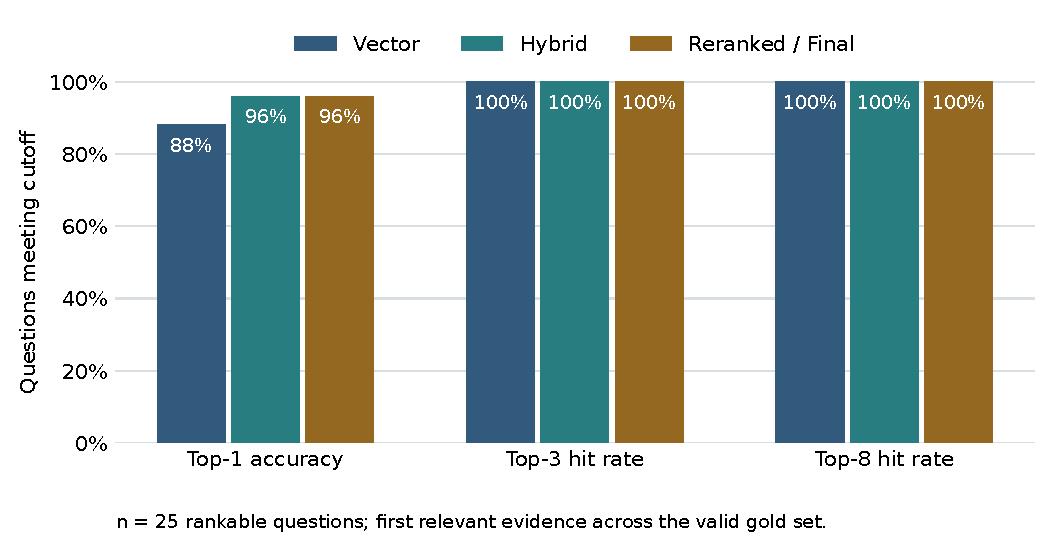
\includegraphics[width=0.98\textwidth]{img/evaluation/evaluation_retrieval_metrics.pdf}
    \caption{Retrieval metrics calculated from the 25 recorded rankable cases. Top-$k$ denotes first-relevant-evidence hit rate; each ordering uses the same applicable questions.}
    \label{fig:eval-retrieval}
\end{figure}

The eight-percentage-point Top-1 improvement corresponds to two cases. Q04 moves the relevant course-notes evidence from vector rank 2 to hybrid rank 1, and Q11 makes the same improvement for the BlueGrid agreement. Both remain first in the final ordering. No further aggregate gain is observed between hybrid and final retrieval.

\subsection{Answers, citations, and safe responses}

Table~\ref{tab:grounding-results} reports 31 correct answers out of 32 (96.9\%) and 28 correct citation judgements out of 29 applicable questions (96.6\%). Both failures belong to Q21, an open-ended synthesis across documents. The 29-case citation denominator excludes only Q22--Q24; Q26 is included because the displayed security-guidelines source was actually retrieved and its mapping was judged correct.

\begin{table}[!htbp]
    \centering
    \caption{Answer and citation results for the completed question set.}
    \label{tab:grounding-results}
    \begin{tabular}{L{0.40\textwidth} L{0.29\textwidth} C{0.20\textwidth}}
        \toprule
        \textbf{Aspect} & \textbf{Assessment unit} & \textbf{Result} \\
        \midrule
        Answer correctness & All 32 questions & 31/32 (96.9\%) \\
        Citation correctness & 29 applicable questions & 28/29 (96.6\%) \\
        \bottomrule
    \end{tabular}
\end{table}

All five no-evidence/security cases pass their recorded checks (Table~\ref{tab:security-results}). Q22--Q24 avoid inventing a gateway Wi-Fi password, an invoice VAT rate, or a chief executive's name. Q25 treats the embedded instruction example as untrusted content. Q26 refuses the request to reveal a secret; its \texttt{S1} citation maps to a real retrieved source rather than one fabricated to satisfy the requested identifier.

\begin{table}[!htbp]
    \centering
    \caption{Observed no-evidence and security responses. Q25 also belongs to the retrieval set.}
    \label{tab:security-results}
    \begin{tabular}{L{0.46\textwidth} L{0.22\textwidth} C{0.20\textwidth}}
        \toprule
        \textbf{Case group} & \textbf{Questions} & \textbf{Result} \\
        \midrule
        Absent-fact abstention & Q22--Q24 & 3/3 (100\%) \\
        Document injection example & Q25 & 1/1 (100\%) \\
        Direct secret request & Q26 & 1/1 (100\%) \\
        Combined assessment & Q22--Q26 & 5/5 (100\%) \\
        \bottomrule
    \end{tabular}
\end{table}

\begin{figure}[!htbp]
    \centering
    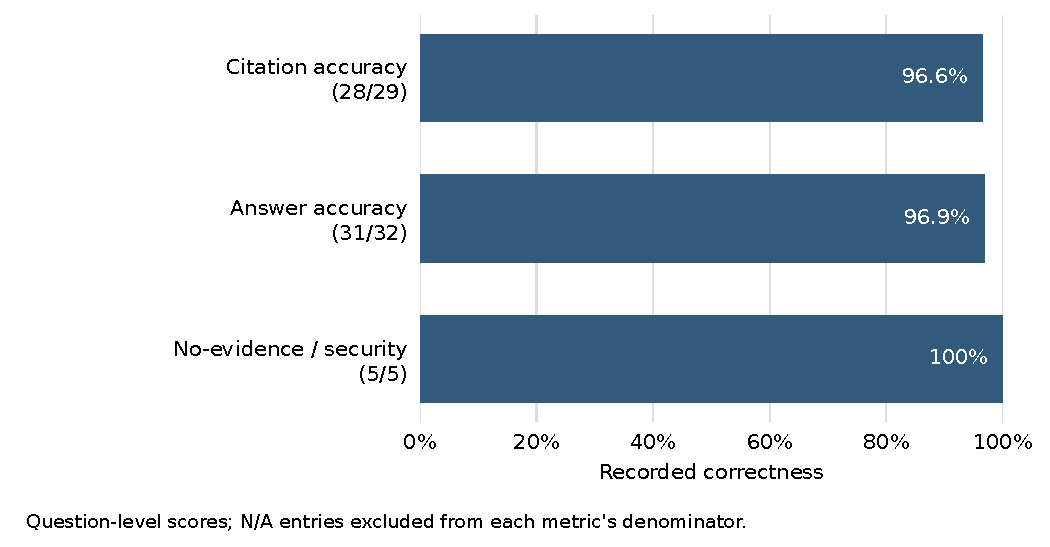
\includegraphics[width=0.98\textwidth]{img/evaluation/evaluation_answer_metrics.pdf}
    \caption{Answer, citation, and no-evidence/security results. The denominators are 32, 29, and 5 respectively; citation judgements are at question level.}
    \label{fig:eval-grounding}
\end{figure}

Figure~\ref{fig:eval-grounding} presents these related response measures without combining their different denominators. The safety total establishes the expected behavior in the five recorded cases, not a general security guarantee.

\subsection{Document Understanding}

M10 obtains the expected controlled type on seven of eight documents (87.5\%) and the expected primary language on all eight (100\%), as shown in Table~\ref{tab:understanding-results}. The only type mismatch is \texttt{08\_edge\_gateway\_manual.pdf}: the gold label is \texttt{TechnicalDocument}, while the application returns \texttt{Manual}. The latter is a plausible description of the content, but it remains an error under the exact-match criterion.

\begin{table}[!htbp]
    \centering
    \caption{Document Understanding results for the eight primary documents.}
    \label{tab:understanding-results}
    \begin{tabular}{L{0.36\textwidth} L{0.34\textwidth} C{0.18\textwidth}}
        \toprule
        \textbf{Task} & \textbf{Metric} & \textbf{Result} \\
        \midrule
        Controlled document type & Exact-match accuracy & 7/8 (87.5\%) \\
        Primary language & Exact-match accuracy & 8/8 (100\%) \\
        \bottomrule
    \end{tabular}
\end{table}

The notes describe strong metadata coverage across the eight cases, including agreement and invoice identifiers, parties, dates, the quarterly reporting period, and the gateway's product and revision. This is qualitative evidence of useful document descriptions. It does not support numerical claims about metadata precision, recall, or title quality.

\subsection{Technical PDF classification and selective OCR}

All three control PDFs receive the expected technical document label (Table~\ref{tab:pdf-classification-results}). The recorded page composition agrees with their construction: three native-text pages in document 09, three scanned pages in document 10, and two native-text pages with one scanned page in document 11. The reported M11 score is three document-level passes, rather than a separately measured page-level confusion matrix.

\begin{table}[!htbp]
    \centering
    \caption{M11 technical classification of the three equivalent control PDFs.}
    \label{tab:pdf-classification-results}
    \begin{tabular}{L{0.39\textwidth} L{0.34\textwidth} C{0.16\textwidth}}
        \toprule
        \textbf{Control document} & \textbf{Expected / actual type} & \textbf{Result} \\
        \midrule
        09: text-based PDF & TextBased / TextBased & Pass \\
        10: scanned PDF & Scanned / Scanned & Pass \\
        11: mixed PDF & Mixed / Mixed & Pass \\
        Overall & Document-level pass rate & 3/3 (100\%) \\
        \bottomrule
    \end{tabular}
\end{table}

\begin{table}[!htbp]
    \centering
    \caption{M12 selective OCR observations. The workbook records a combined routing/content pass for each control.}
    \label{tab:ocr-results}
    \begin{tabular}{L{0.24\textwidth} L{0.22\textwidth} L{0.20\textwidth} C{0.20\textwidth}}
        \toprule
        \textbf{Control} & \textbf{OCR status} & \textbf{OCR pages} & \textbf{M12 result} \\
        \midrule
        09: text-based & Not required & None & Pass \\
        10: scanned & Ready & 1, 2, 3 & Pass \\
        11: mixed & Ready & 2 only & Pass \\
        Overall & --- & --- & 3/3 (100\%) \\
        \bottomrule
    \end{tabular}
\end{table}

Table~\ref{tab:ocr-results} shows that OCR was avoided for the native control, completed for all three scanned pages, and limited to page 2 of the mixed control. The latter retained native pages 1 and 3. These observations support selective routing in the tested layouts. M12's three passes include the native control, so 3/3 must not be read as three successful transcription tests.

The final Q13 run and Q29--Q32 obtain correct answers with first-relevant evidence at rank 1. The recovered facts include the site code RAVEN-7319, the monthly maintenance window, the 15-minute acknowledgement period, and escalation reference ESC-441-A. In Q31, the answer correctly states that the memo does not specify the action to take after an interruption continues beyond 04:15; the notes also record mention of a separate Priority 1 procedure. Its recorded pass concerns preserving that limitation rather than inventing the missing instruction.

\begin{figure}[!htbp]
    \centering
    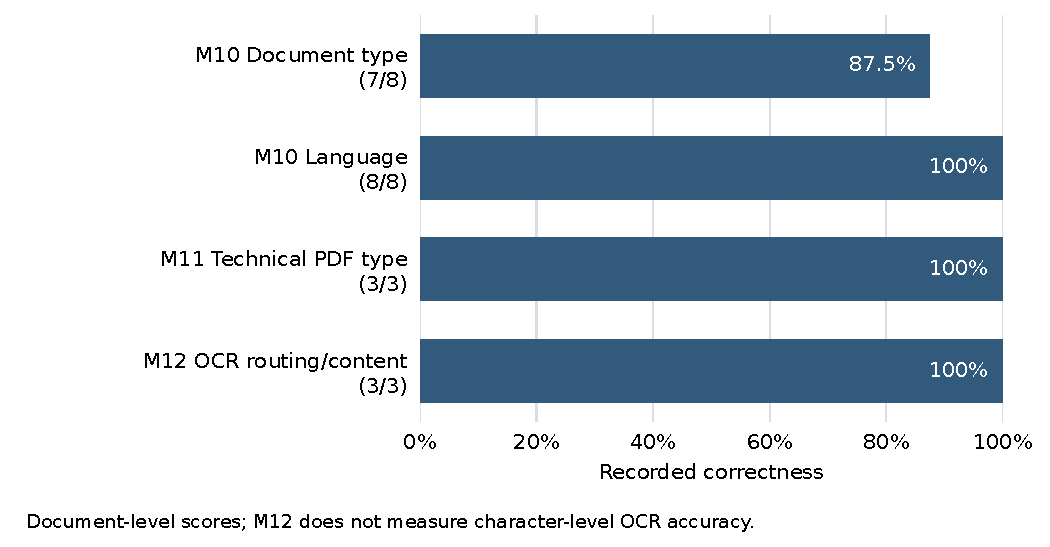
\includegraphics[width=0.98\textwidth]{img/evaluation/evaluation_document_processing_metrics.pdf}
    \caption{Document-processing results with their separate denominators: M10 type and language use eight primary documents; M11 and M12 use three control PDFs. M12 is a recorded combined routing/content pass rate, not character-level OCR accuracy.}
    \label{fig:eval-classification}
\end{figure}

Figure~\ref{fig:eval-classification} brings together the available processing measures while preserving the distinction between semantic labels, technical classification, and the combined OCR assessment. No aggregate across these tasks is calculated.

\section{Discussion}
\label{sec:evaluation-discussion}

\subsection{Ranking improvements and answer completeness}

The observed hybrid advantage is modest and specific: two additional questions have relevant evidence in first position, with no change to Top-3 or Top-8 coverage. Evidence within the first three positions makes it available early in the candidate ordering, although the answer generator must still select and interpret it correctly. Q04 concerns a conceptual RAG explanation, while Q11 contains the exact BlueGrid agreement identifier. The workbook attributes their promotion to hybrid retrieval and, for Q11, notes metadata involvement. These observations are compatible with complementary retrieval signals helping different query forms, but there is no isolated lexical or metadata ablation from which to assign their individual contributions.

The final stage neither improves nor worsens the reported retrieval metrics relative to hybrid retrieval. This sample therefore provides no measured aggregate gain from reranking. It also does not establish that reranking is ineffective in larger or more ambiguous collections, particularly because application/fallback status and repeated runs are not documented.

Q28 illustrates why first-position ranking and answer correctness require separate evaluation. The evidence about service credits preserving termination rights remains at rank 2 in every ordering. Nevertheless, the answer correctly uses the relevant \texttt{S2} evidence. This is a Top-1 miss with a correct answer, rather than a complete retrieval or generation failure.

Q21 is the principal observed answer failure. It asks which documents mention Meridian Retail and what role the organization has in each. The expected set contains the NovaTel agreement and invoice, where it is the customer; the BlueGrid agreement, where it is the client; and the quarterly report, which it issues. The response identifies several roles correctly but also includes a document where Meridian Retail is absent, notably the tax-residency policy. Both answer and citation correctness are therefore marked No. Partial correctness does not compensate for the unsupported inclusion in an otherwise apparently comprehensive synthesis. This case shows that the presence of citations alone does not ensure correct evidence selection or semantic support.

This contrasts with Q19 and Q20, where focused comparisons correctly combine the two required sources. The pattern suggests that broad entity-based enumeration is a more demanding task than a comparison with explicitly named documents. The workbook establishes over-broad aggregation in Q21 but does not expose enough detail to identify whether the decisive error arose during retrieval, context selection, or answer generation. A future evaluation of such questions would need to score both coverage of the required source set and unsupported inclusions.

\subsection{Processing and safety interpretation}

The M10 mismatch shows the practical importance of the controlled-label definition. \texttt{Manual} describes the gateway document plausibly, yet differs from the required \texttt{TechnicalDocument} label. Retaining it as an error avoids revising the gold standard after observing the prediction. Correct language labels and useful metadata notes are encouraging within this corpus, but do not establish broad multilingual or entity-extraction performance.

The PDF controls demonstrate the intended distinction between native, scanned, and mixed content, including selective OCR of a single scanned page. The strongest direct evidence concerns routing and preservation of native pages. The equivalent control sources and absence of a transcription score prevent a claim that OCR is perfectly accurate. Similarly, the five successful no-evidence/security responses show appropriate abstention and handling of the tested instructions, but do not quantify robustness against a wider attack distribution.

\subsection{Threats to validity}

\textbf{Internal validity.} Gold expectations and pass/fail judgements are manually recorded, and no independent scorer or inter-rater agreement is documented. Binary question-level scoring can conceal differences in partial correctness. Case notes make the principal failure reviewable, but the available records do not support causal attribution to individual retrieval or generation components.

\textbf{External validity.} The evaluation uses 11 synthetic PDFs, of which three repeat equivalent control content. The eight primary documents cover a limited range of domains and only English and Romanian primary-language labels. Clear synthetic identifiers and controlled content may be easier than noisy, long, or heterogeneous production collections. The experiment does not establish performance for DOCX input, ImageBased or Unknown PDF cases, extreme scans, classification threshold boundaries, or the document-understanding sampling limit. Automated tests cover some related implementation risks, but are separate evidence from these application-level results.

\textbf{Construct validity.} First-relevant-evidence hit rate measures access to at least one supporting result, not retrieval of all required evidence. Citation judgements are per question, not an independent claim-level accuracy measurement. M12 combines routing/content observations and includes a case requiring no OCR; it is not a transcription-accuracy estimate. Metadata notes have no precision/recall denominator. These distinctions constrain the meaning of the high percentages.

\textbf{Reproducibility and scope.} Uploads were staged, Q13 was retested, and there is no complete frozen configuration or external model-version record. No repeated trials quantify model variability. The workbook also contains no latency, provider-usage, production-load, historical-citation-snapshot, empty-workspace, or cross-user experimental measurements. The results therefore support correct operation on most recorded cases, with a measurable hybrid Top-1 improvement and a documented failure in broad multi-document synthesis; they do not establish production-scale performance or comprehensive security.
